\chapter{Wybór technologii oraz narzędzi}


\section{Wykrywanie twarzy na zdjęciu}

Wykrywanie twarzy to pierwszy krok w zaprojektowanym systemie.
Z powodu, że jest on umieszczony na samym początku, proces ten musi być maksymalnie skuteczny.
Jeżeli na zdjęciu nie zostanie wykryta twarz, to cały proces zakończy się z negatywnym rezultatem.
\textbf{Twarzy nie będzie można zidentyfikować, jeżeli nie zostanie ona znaleziona.}
Oznacza to, że twarze muszą być wykrywane z różnymi orientacjami, kątami,
poziomem oświetlenia, makijażem, kapeluszami, zarostem, fryzurami, okularami, wiekiem i tak dalej.
Niestety twarz ludzka jest obiektem dynamicznym i ma duży stopień zmienności w wyglądzie,
co sprawia, że wykrywanie twarzy jest trudnym problemem w widzeniu komputerowym~\cite{HJELMAS2001236}.

W artykule z 2016 roku zatytułowanym
``Joint Face Detection and Alignment Using Multitask Cascaded Convolutional Networks''~\cite{zhang2016joint}
została zaproponowana wielozadaniowa kaskadowa konwolucyjna sieć neuronowa
(MTCNN\footnote{Skrót z języka angielskiego od Multi-Task Cascaded Convolutional Neural Networks })
do wykrywania twarzy.
Sieć ta zyskała duża popularność, ponieważ osiągnęła wówczas najlepszy wyniki
w wykrywaniu twarzy na zdjęciach dla wybranych zbiorów danych.
Kolejną zaletą zaproponowanej sieci neuronowej jest to, że jest w stanie rozpoznać punkty orientacyjne twarzy, takie jak oczy, usta i nos.
Wyniki przeprowadzonych eksperymentów w artykule zostały przedstawione na rysunku~\ref{fig:mtcnn_wyniki}.

\begin{figure}[P]
    \centering
    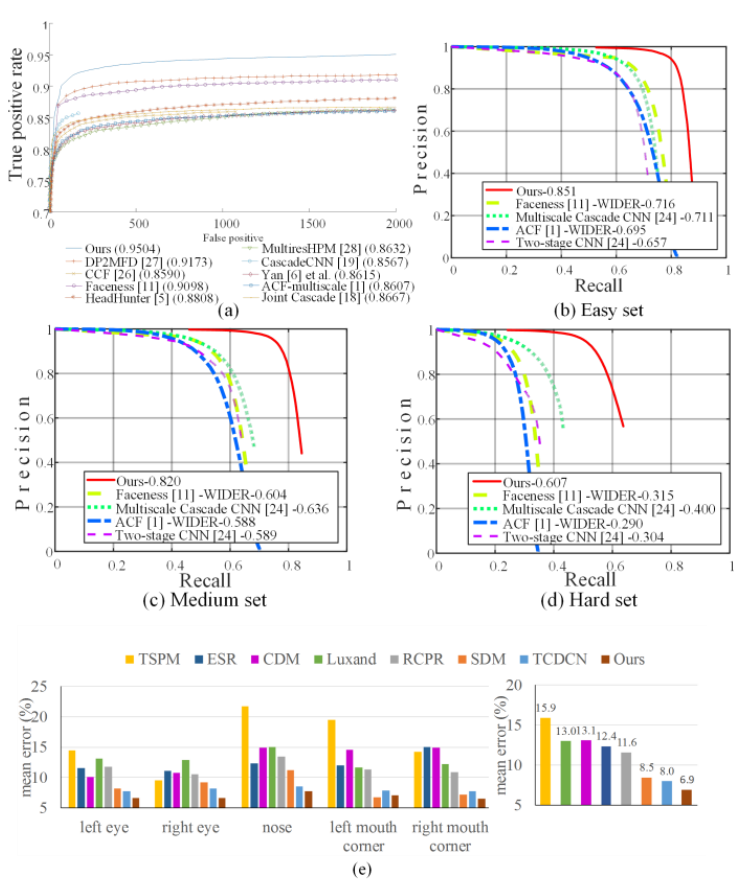
\includegraphics[width=1\textwidth]{images/mtcnn-wyniki}
    \caption{
        Wyniki przeprowadzonych eksperymentów. Słowo ``Ours'' oznacza sieć MTCNN.
        (a) wyniki z testów na bazie FDDB.
        (b-d) wyniki z testów dla trzech kolejnych zbiorów na bazy Wider Face.
        (e) Wyniki z testów dla wyrównania twarzy na bazie AFLW.
    }
    \bibsource{\cite{zhang2016joint}}
    \label{fig:mtcnn_wyniki}
\end{figure}


W internecie znajduje się spora liczba implementacji MTCNN~\cite{mtznn_all_impls}.
Spośród dostępnych została wybrana sieć napisana przez \textit{Iván de Paz Centeno}
i udostępniona na portalu GitHub\footnote{GitHub - dostawcą platformy internetowej do tworzenia
oprogramowania i kontroli wersji za pomocą narzędzia Git udostępniania
pod adresem \url{https://github.com}. } (\url{https://github.com/ipazc/mtcnn}) na zasadach licencji MIT\footnote{Licencja MIT daje użytkownikom
nieograniczone prawo do używania, kopiowania, modyfikowania i rozpowszechniania (w tym sprzedaży)
    oryginalnego lub zmodyfikowanego programu w postaci binarnej lub źródłowej.
    Jedynym wymaganiem jest, by we wszystkich wersjach zachowano warunki licencyjne i informacje o autorze.
}~\cite{ipazc/mtcnn}.
Główną zaletą wybranego narzędzia jest łatwość użycia.
Sieć została napisana w języku programowania python w bibliotece TensorFlow
i całość udostępniona jako pakiet z możliwością instalacji
przez PIP\footnote{PIP - narzędzie do instalowania pakietów python}.


\section{FaceNet}

FaceNet to architektura, oparta na głębokiej sieci neuronowej, która bezpośrednio uczy się mapowania
z obrazów twarzy do zwartej przestrzeni euklidesowej,
w której odległości bezpośrednio odpowiadają mierze podobieństwa twarzy~\cite{schroff2015facenet}.
Wynikiem działania sieci jest wektor składający się z elementów charakteryzujący daną twarz.
Długość wektora jest zależna od konkretnej implementacji.
Po utworzeniu przestrzeni euklidesowej na bazie dostępnych zdjęć twarzy,
zadania polegające na identyfikacji, weryfikacji czy grupowaniu
sprowadzają się do pomiaru odległości pomiędzy poszczególnymi wektorami cech~\cite{schroff2015facenet}.
Wizualizacja procesu mapowania zdjęcia do przestrzeni
euklidesowej została przedstawiona na rysunku~\ref{fig:facenet_zastosowanie}.

\begin{figure}[]
    \centering
    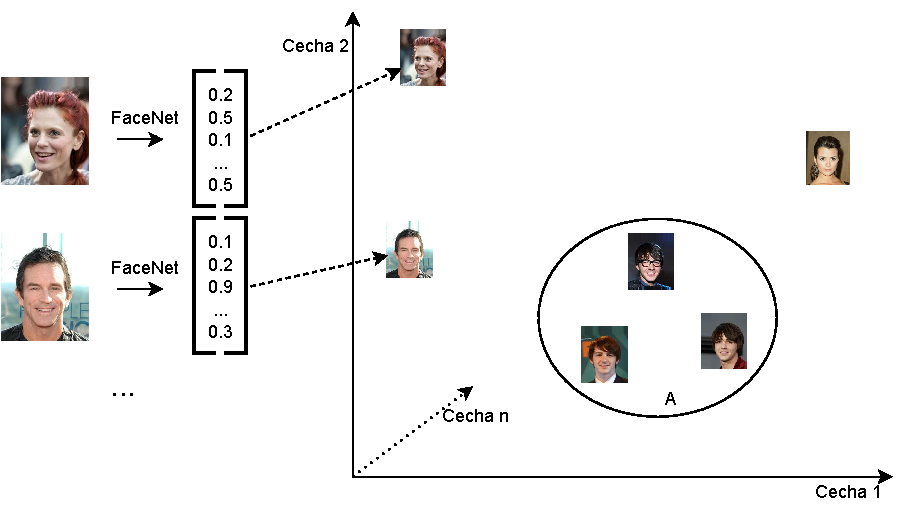
\includegraphics[width=1\textwidth]{images/facenet_euc}
    \caption{
        Proces umieszczania wektorów cech w przestrzeni euklidesowej.
        Zdjęcia przedstawiające tę samą osobę znajdą się bliżej siebie względem zdjęć innych osób.
        Literą ``A'' zostały oznaczone zdjęcia przedstawiające tę samą osobę.
    }
    \customsource
    \label{fig:facenet_zastosowanie}
\end{figure}

\subsection{Zasada działania}

FaceNet pobiera obraz twarzy osoby jako dane wejściowe i wyprowadza wektor,
który reprezentuje najważniejsze cechy twarzy (wektor cech).
Operacje ta, jest pewnego rodzaju kompresją, której zadaniem jest zmniejszenie ilości informacji
na temat danej rzeczy (w tym wypadku zdjęcia twarzy) bez utraty kluczowych informacji.
Informacje, jakie są pobierane ze zdjęcia, nie są z góry zdefiniowane.
Za odpowiedni dobór parametrów jest odpowiedzialna głęboka sieć neuronowa, która traktowana jest
jako czarna skrzynka, czyli miejsce, gdzie znane są tylko dane wejściowe oraz dane wyjściowe.
Oznacza to, że nie są znane parametry, które są pobierane ze zdjęcia, a wartości w wektorze cech,
generowane na wyjściu, są trudne, o ile w ogóle możliwe, do zinterpretowania.

Oprócz samej sieci neuronowej FaceNet składa się również z innych warstw, normalizacji L2 oraz
funkcji strat \textit{triplet loss} (rysunek~\ref{fig:facenet_arch}).
Normalizacja L2 polega na takim zmodyfikowaniu wartości otrzymanego zbioru, aby w każdym wierszu
suma kwadratów była zawsze równa $1$,
natomiast zadaniem funkcji \textit{triplet loss} jest, w procesie trenowania sieci,
minimalizowanie odległości pomiędzy prawdziwymi
wyrażeniami oraz maksymalizowanie dla fałszywych~\cite{chechik2010large}.
Innymi słowy, celem jest, aby odległości między wektorami tych samych osób były jak najmniejsze,
a odległości pomiędzy wektorami różnych osób --- maksymalne.
Zasada działania funkcji \textit{triplet loss} w sposób graficzny
została przedstawiona na rysunku~\ref{fig:triplet_loss}.

\begin{figure}[]
    \centering
    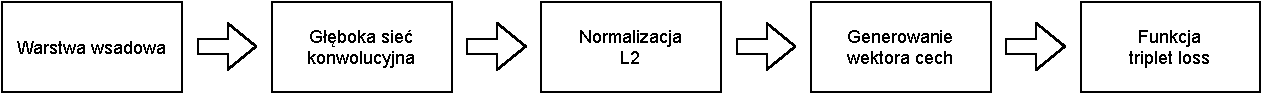
\includegraphics[width=1\textwidth]{images/facenet_arch}
    \caption{ Architektura FaceNet z podziałem na poszczególne warstwy }
    \customsource
    \label{fig:facenet_arch}
\end{figure}

\begin{figure}[]
    \centering
    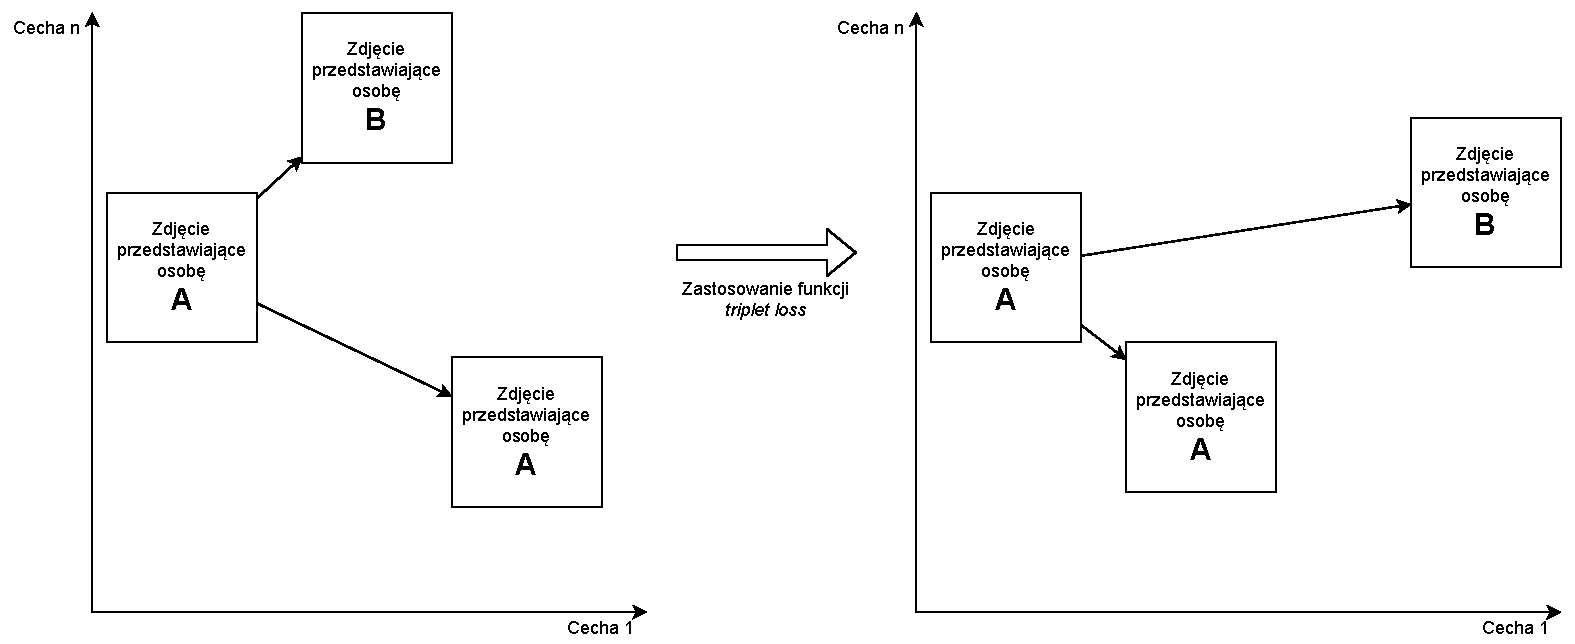
\includegraphics[width=1\textwidth]{images/triplet_loss}
    \caption{ Uproszczony schemat obrazujący zasadę działania funkcji strat \textit{triplet loss} }
    \customsource
    \label{fig:triplet_loss}
\end{figure}

Całość procesu uczenia się sieci FaceNet, można zatem w uproszczeniu, podsumować w następujących krokach:

\begin{enumerate}
    \item zdefiniowanie parametrów początkowych sieci,
    \item wygenerowanie wektorów cech twarzy,
    \item użycie funkcji strat \textit{triplet loss},
    \item dostosowanie się parametrów sieci tak, aby przykład pozytywny był bliżej zdjęcia wzorcowego, niż przykład negatywny,
    \item powrót do kroku drugiego tak długo, aż zwracane wektory osiągną zadaną dokładność
\end{enumerate}

\subsection{Wpływ wielkości zdjęcia na działanie sieci}

W pracy pod tytułem \textit{Facenet: A unified embedding for face recognition and clustering}~\cite{schroff2015facenet}
została wytrenowana sieć o architekturze FaceNet na zdjęciach w formacie JPEG o rozmiarach 220 na 220 pikseli.
Podczas testowania wytrenowanej sieci, po dostarczeniu zdjęć o mniejszych rozmiarach (względem rozmiarów
zdjęć, na których sieć była trenowana) okazało się, że sieć ta jest również bardzo skuteczna.
Sieć miała akceptowalną skuteczność nawet po dostarczeniu zdjęć o rozmiarach 80 na 80 pikseli.
Trenowanie sieci na zdjęciach o mniejszej rozdzielczości mogłoby jeszcze poprawić ten wynik.
Dokładne informacje na temat wpływu liczby pikseli na
trafność sieci zostały przedstawione w tabeli~\ref{tab:quality_pixels_to_rate}

\begin{table}[]
    \caption{Wpływ jakości zdjęcia oraz liczby pikseli na trafność sieci FaceNet. Źródło: \cite{schroff2015facenet}}
    \label{tab:quality_pixels_to_rate}
    \begin{minipage}{.5\linewidth}
        \centering
        \begin{tabular}{|l|l|}
            \hline
            Liczba pikseli                & Trafność \\ \hline
            1 600 \hspace{15px} (40x40)   & 37.8\%   \\ \hline
            6 400 \hspace{15px}     (80x80)    & 79.5\%   \\ \hline
            14 400 \hspace{10px}  (120x120) & 84.5\%   \\ \hline
            25 600 \hspace{10px}  (160x160) & 85.7\%   \\ \hline
            65 536 \hspace{10px}  (256x256) & 86.4\%   \\ \hline
        \end{tabular}
    \end{minipage}%
    \begin{minipage}{.5\linewidth}
        \centering
        \begin{tabular}{|l|l|}
            \hline
            Jakość JPEG & Trafność \\ \hline
            10          & 67.3\%   \\ \hline
            20          & 81.4\%   \\ \hline
            30          & 83.9\%   \\ \hline
            50          & 85.5\%   \\ \hline
            70          & 86.1\%   \\ \hline
            90          & 86.5\%   \\ \hline
        \end{tabular}
    \end{minipage}
\end{table}

\subsection{Użycie wytrenowanej sieci}

W projektowanym systemie zostanie użyty wstępnie wytrenowany model \textit{Keras FaceNet}~\cite{taniai-2018},
który został wyszkolony na bazie zdjęć dostarczonych przez MS-Celeb-1M~\cite{microsoft-2020-celeb1m}
i udostępniony przez \textit{Hiroki Taniai}~\cite{taniai-no-date}.
Dostarczane zdjęcia twarzy powinny być kolorowe, w formacie RGB oraz
o rozmiarach 160 pikseli na 160 pikseli~\cite{brownlee-2019}.


\section{Kadrowanie i standaryzacja}

Do przetwarzania plików graficznych zostanie wykorzystana biblioteka \textit{PILLOW} napisana w języku python.
Biblioteka wspiera wiele formatów graficznych,
w tym te najpopularniejsze jak \textit{PNG}, \textit{GIF}, \textit{JPEG} oraz \textif{BMP}~\cite{pillow_doc},
dzięki czemu nie będzie wymagane, aby użytkownik sam konwertował plików graficznych do odpowiedniego formatu.
Biblioteka \textit{PILLOW} zostanie również wykorzystana do wycinania zdjęcia twarzy oraz standaryzacji
i normalizacji już wykadrowanego zdjęcia.


\section{Obsługa systemu}

Całość zaprojektowanego systemu ma być dostępna z przeglądarki internetowej.
Aby sprostać temu wymaganiu, należy napisać usługę, która jest w stanie obsługiwać połączenia
HTTP\footnote{Skrót z języka angielskiego od słów Hypertext Transfer Protocol}.
Z powodu, że narzędzia do wykrywania twarzy, obróbki zdjęć oraz FaceNet są udostępnione w języku python,
program zostanie również napisany w tym języku.
Oprócz samej strony internetowej potrzebna jest również baza danych,
w której będą przechowywane informacje o dostępnych zdjęciach.
Same zdjęcia będą przechowywane na serwerze plików.
Sporym ułatwieniem będzie również panel umożliwiający zarządzanie dostępnymi zdjęciami w systemie.

Narzędziem, które spełni wyżej postawione wymagania jest platforma programistyczna \textit{Django},
która umożliwia w łatwy sposób zarządzanie bazą danych za pomocą mapowania obiektowo-relacyjnego,
pozwala na zarządzanie danymi dostępnymi w bazie danych poprzez panel administratora, dostępny
z poziomu przeglądarki oraz co najważniejsze, jest napisana w języku python~\cite{djangodoc}.